\chapter{城市内部复杂现象的物理解释}

我们长久以来知道城市的优势在于规模效应。城市增长与发展规律就成为了研究城市命运的一个重要内容\cite{thisse2010toward}。Bettencourt和West在\cite{bettencourt2010unified}中讲述了城市优势的具体形式:超线性增长,即城市指标的增益随城市规模的增加呈现超线性的趋势。Barthelemy在\cite{Barthelemy2019}中讲述了城市结构的诸多方面,既有好的方面,比如城市的创造力\cite{Arbesman2009};也有坏的方面,比如城市中传染病的发病率\cite{PhysRevE.94.052316}和犯罪率\cite{banerjee2015competitive}也在城市规模增大的过程中增加了。

\begin{figure}
  \centering
  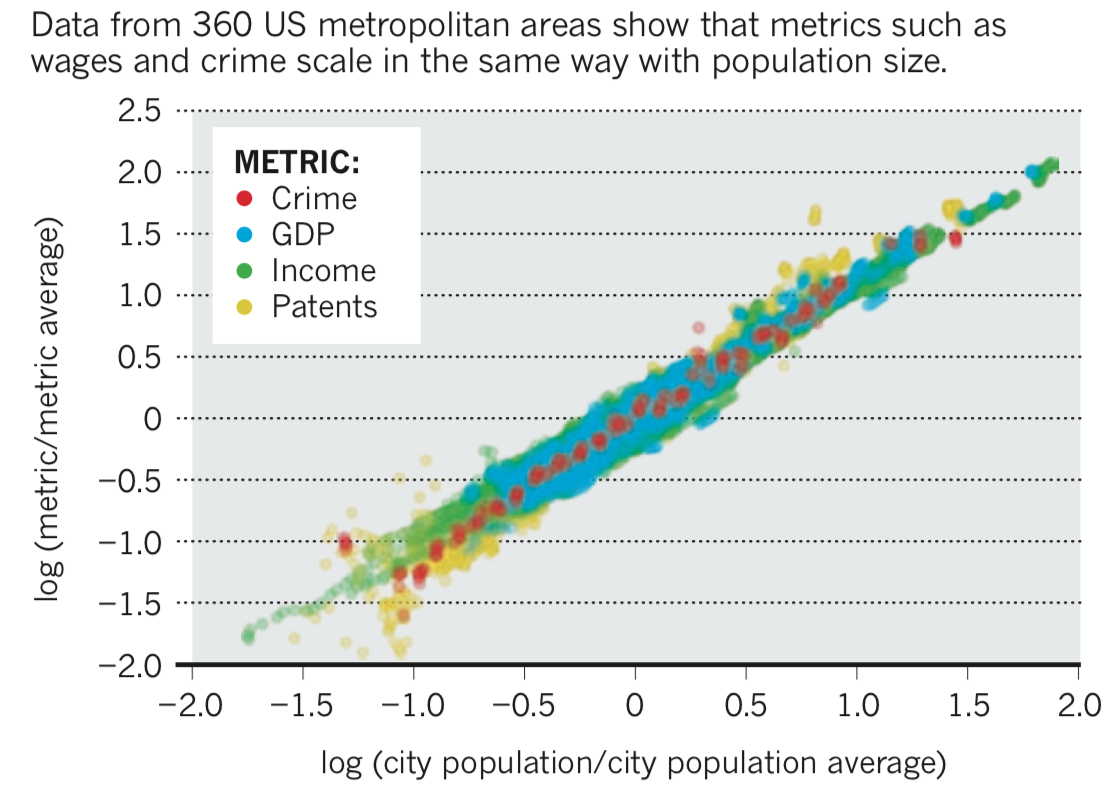
\includegraphics[width = \linewidth]{pictures/scaling.png}
  \caption{Bettencourt和West\cite{bettencourt2010unified}。360个美国城市中各项指标与城市人口之间的关系。我们可以看出,城市越大,无论是商品,资源还是观念,普通公民拥有,生产和消费的东西就越多。平均而言,随着城市规模的扩大,人均社会经济数量,例如工资,GDP,生产的专利数量和教育和研究机构的数量都在增加,而且比预期的线性增长高出约15%。}
\end{figure}

与此同时,城市基础设施建设是一个自上而下的,需要用有限资源覆盖尽量大的区域的问题\cite{PhysRevE.90.022803,PhysRevE.74.016117}。空间选址问题的解显示,最优配置的密度是亚线性的,即基础设施的数量的增加比城市规模的增加要慢。在\cite{PhysRevE.74.016117}中,作者讨论了在人口密度不均的国家/地区建造医院,机场或购物中心之类的设施,以使人的住所到最近的设施的平均距离最小。我们回顾了此问题的一些先前近似处理,这些处理表明,设施的最佳分布应具有随人口密度增加的密度,但其速度要比线性慢(三分之二)。该结论通常可以用两种方法来验证,即回归分析方法,和基于密度依赖的地图投影方法。不同的基础设施的能覆盖的空间面积也是不同的。不同基础设施和产业的相互支持关系使得城市功能形成了一个生态系统。每个城市在不同产业的不同层次承担了不同的任务\cite{camagni1993city,christopherson1986city}。在\cite{PhysRevE.74.016117}还提出了空间设施之间的交互问题。例如机场建设起来后,我们还需要研究机场之间的航班网络。其中处理的方法是建立成本度量,进而使网络维护和旅行的总成本最小化。这可以给我们一些经济方面的启示。在资源配置的时候,不只是资源支持人的生活,亦是资源支持其他产业的生产。

城市研究中,在空间和经济投入限制情况下的动态生长状况一直是难以预测的。我们将首先以交通为线索,讲述城市内部亚线性的导出模型。随后我们将对城市生态系统的性质展开讨论,并给出几个理想的进展方向。城市要素在空间上存在着交互。通过对城市内部交互进行建模可以得到城市的很多规律的物理解释。城市增长规律的超线性性和同级别城市基础设施建设的亚线性性就是典型的例子。但这种解释是否是第一性的还有待研究。本章试图整理空间交互在解释城市内部尺度的现象的工作,并给出一些已有结构的限制条件下,空间交互适应环境的一个优化模型。

\section{城市形态与随机几何模型}

与其他地理现象一致,城市的发展也会受到地形、已有人类活动分布的限制和影响。Courtat在\cite{Courtat2011}中所言,局部的地理环境可以被比作限制城市发展的壳。所以城市在形态学上形式各异,已知的任何模型都不能将城市的几何、功能、和动力学过程纳入统一的可预测框架之中。\cite{Courtat2011}中的模型利用街道和城市性质进行建模,假设城市的发展遵循空间划分或扩展的逻辑,并提出了一种动态模型,该模型可以模仿这种逻辑,并且可以通过简单的一般规则和一些参数成功地产生大量的城市多样性并重现静态分析所指出的一般特征。

这一工作将城市简化为街道段地图,并表明我们可以基于这种几何与拓扑表示推导出很多城市信息,而无需人口分布、街道宽带等的附加数据。当我们将城市当作一个图来理解时,我们可以挖掘出城市的几何特征,其拓扑特征可以作为构建城市形态的骨架。尽管城市总体形状不同(一阶拓扑各向异性),仍存在一些基本的规则可以解释城市的普遍形态。城市基础设施的分布适应于不同地区的局部地理环境,满足当地人们的居住需求并同时保持高效的城市通行。这一工作提出的基于空间划分或扩展的模型提取了超越局部因素限制与动态行为的城市结构特征。例如,生成的街道系统的对数缩放具有全局性和非平凡属性,可以验证模型并适用于观察到的较小的拓扑半径中。城市形态的生成过程实现了对空间的划分和扩展,通过模型的调整和结果比较,验证了这一过程对城市建模具有鲁棒性。

空间尤尔模型在这个问题中也有着很好的对应。如果我们将模型中的占领机制忽略掉,在时间趋于无穷的时候,二维欧氏空间上的单个社区的生长会趋向于一个圆盘的形状。但是,如果我们考虑空间占领的机制,情况就会发生改变。这使得几个区域之间的边界呈现出分型模式。这也与国与国之间形成的自然边界是类似的。所以空间尤尔模型的局部博弈机制也可以解释区域之间边界的分型特征:这些是由确定了具体归属的微观层面的竞争机制导致的。

另一方面,不只是城市景观,城市活动在空间上也存在者分异性特征。\cite{hierarchicalorganization}给出了一种结构指标。这种结构指标给出了人类移动性和城市宜居程度的关系。更强流动性的城市的市民使用公共交通的比例更高,城市功能更加分散,城市更加扁平,宜居性也越强。

\begin{figure}
  \centering
  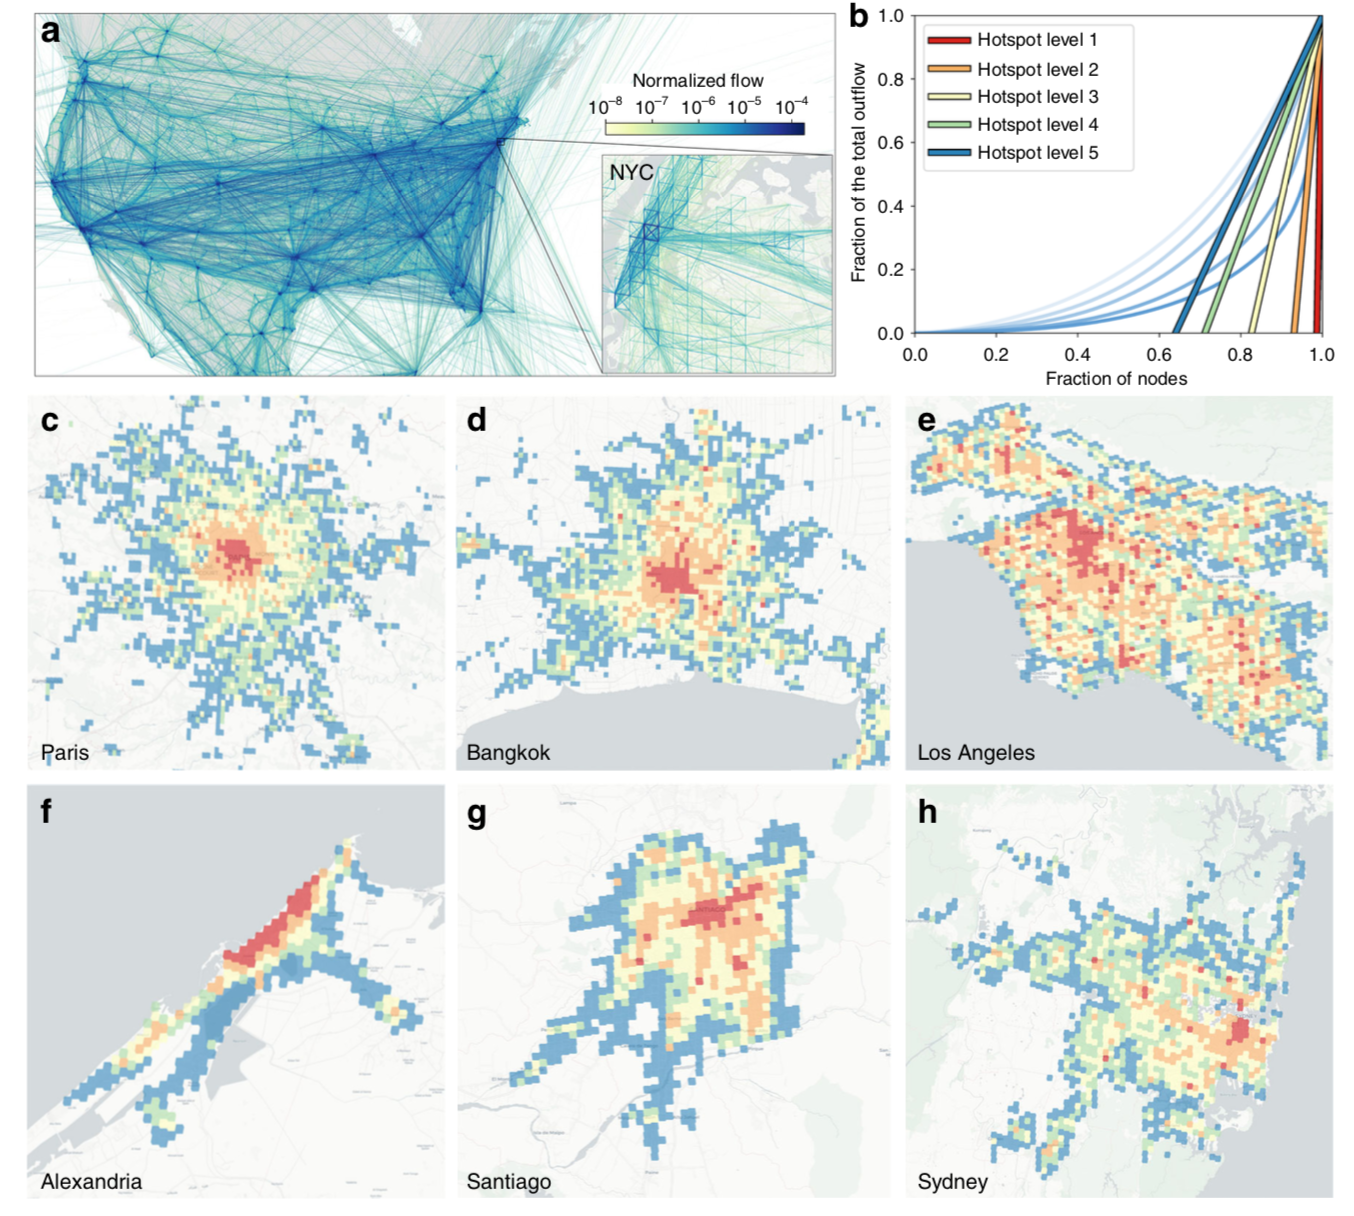
\includegraphics[width = \linewidth]{pictures/h1.png}
  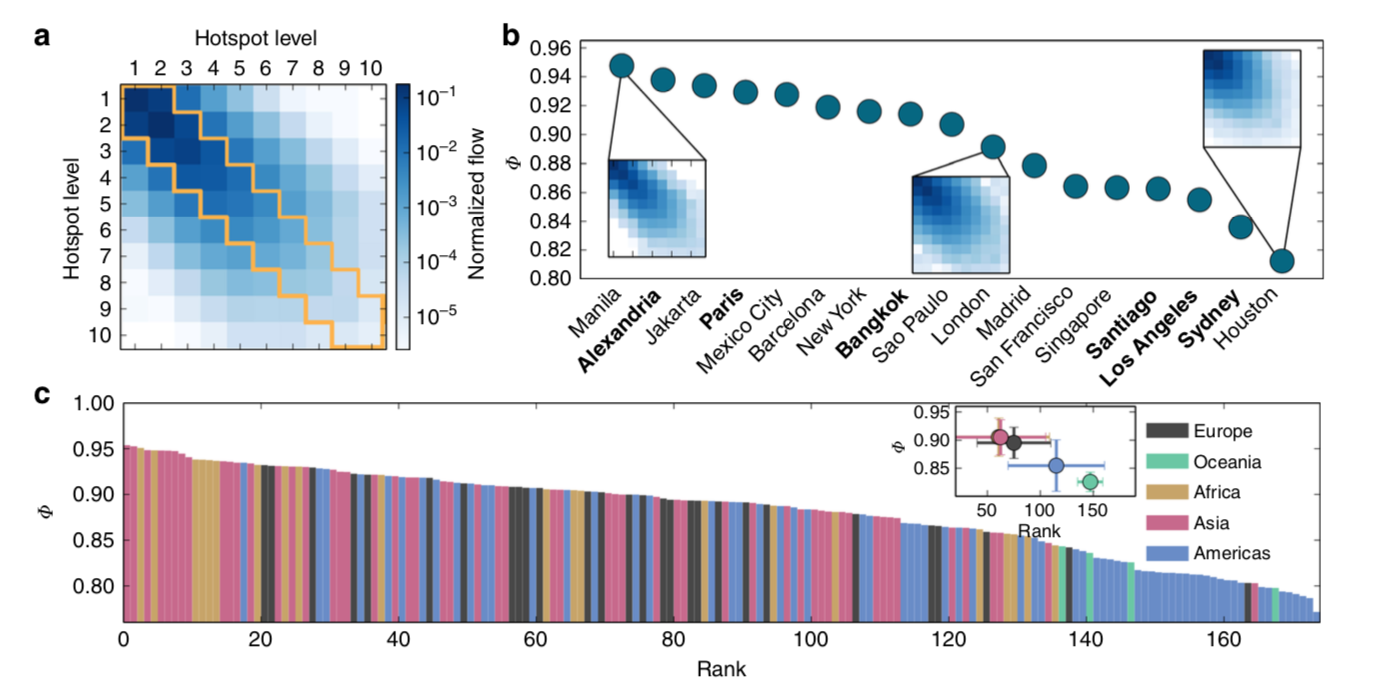
\includegraphics[width = \linewidth]{pictures/h2.png}
  \caption{上图是城市热点分析。下图是城市热点层级结构与\cite{hierarchicalorganization}中指标的相关性。文中进一步解释了集中性与城市宜居性之间的负相关关系。}
\end{figure}

\cite{Weiner17874}中的模型描述了自然竞争机制下空间分异和异质性人群演化的规律。模型中不同群体占据不相重叠的空间,而营养物质则在空间中随机扩散。结果表明:养分扩散速度是生物多样性和人口变化的时间尺度的重要参数。营养物质的快速扩散使某些物种的种群移动的收益为零,从而导致物种灭绝。此外,领土竞争会自发地产生多重稳定性,因此小规模的扰动会对生态产生重大影响。空间中对资源的竞争使得更多的种群可以共存。这个数学模型在理论上解释了城市复杂的形态和高速的流动性使得城市尺度上可以保留产业的多样性。

城市空间分隔也存在着一些物理背景。1971年,Schelling提出了一种模型,如果有太多相反类型的邻居,他们的家庭就会搬家。在\cite{Durrett14036}中,考虑了模型的一个总体种群版本,其中将一个城市划分为N个街区,每个街区都有L座房屋。对于某些$\rho <1/2$,有$\rho NL$红色种族和$\rho NL$蓝色种族。如果邻里有对等类型的$≤\rho cL$个家庭,他们会感到幸福,否则,他们会感到不高兴。每个家庭搬到每个空置房屋的速度取决于他们当前所在位置和目的地的幸福感。我们的主要结果是,如果邻域较大,则将存在临界值$\rho b<​​\rho d<\rho c$,因此对于$\rho <\rho b$,这两种类型会随机地均衡分布。当$\rho >\rho b$时,出现一个新的隔离平衡。对于$\rho b<\rho <\rho d$,存在双稳态,但是当$\rho $超过$\rho d$时,随机状态不再稳定。当$\rho c$足够小时,当$\rho $接近$1/2$时,随机状态将再次成为平稳分布。如果是这样,则在其之前是双稳态区域。该工作的结果显示,城市空间物理分隔的机理性解释不一定存在。不同的城市模式可能只是相同的初始状态被轻微扰动后得到的模式。

Makse, Havlin和Stanley在1995年引领了Diffusion-limit aggregation(DLA)模型在城市科学中的研究\cite{MakseModelling}。该模型认为城市的增长方式可能类似于二维粒子聚集体的增长,也有几篇工作\cite{doi:10.1111/j.1538-4632.1991.tb00245.x, BENGUIGUI199513}使用聚类统计物理学的思想对城市增长进行建模。DLA模型预测应该只存在一个大的分形城市,并且可以不使用传入的“发展单位”(例如,代表人员,资金或资源),因此集群的几乎所有增长都发生在城市边缘的尖端。该工作改进了DLA模型。其中与发展单位相关而不是随机添加到集群中的模型,能够更好地再现观察到的城市形态和城市中子集群(“城镇”)的区域分布系统,也可以描述城市增长动态。该模型与存在密度梯度时的相关渗滤模型相对应,其出发点是城市地区的发展吸引了进一步的发展。该模型提供了预测城市形态的全局属性(例如标度律行为)的可能性。

笔者对城市仅在边缘生长和城市自然生长进行了数值模拟,得到了相似的模式图案。
\begin{figure}
  \centering
  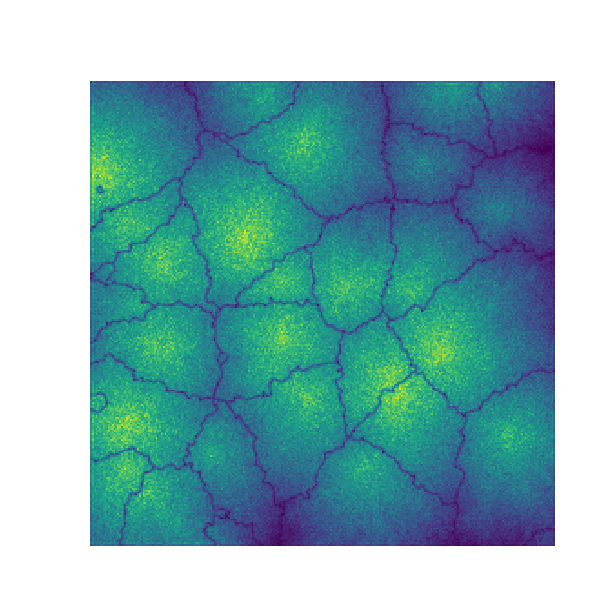
\includegraphics[width = \linewidth]{pictures/fractal_41_256.pdf}
  \caption{仅仅假设边缘增长情形下,由SYM模型生成的的城市模式。浅色代表高人口密度。}
\end{figure}

\section{城市交通系统的性质}

城市交通系统是理解城市内动态的重要切入点。从短时间尺度来看,交通可达性决定了城市建设可能的通行范围,交通拥堵的舒缓的理论解释也是所有人关注的焦点之一;长时间尺度来看,交通网络可以联系物质空间上的价值分布,所以交通网络的性质对塑造城市形态,尤其是多中心性,有着重要的指导意义。

城市交通系统是难以研究的。以路面交通的单一路段来说,路段的流量与速度之间是非线性关系。增加路网通勤效率与建设成本通常也是矛盾的\cite{GulyNavigable}。我们有必要处理细微变化对交通系统的影响,所以需要引入弹性的概念。弹性在自然和工程系统中都有很广泛的应用。它表示了系统从不同的干扰中适应和恢复的能力。尽管弹性是一个在交通系统中管理风险和理解其是如何崩溃的重要概念,但是这个概念在交通系统中的定义和它的统计性质还是缺失的。\cite{Zhang8673}基于交通堵塞的时空组团,定义了城市中交通弹性的概念。并发现,在2维城市路网和1维高速公路中,弹性的概率分布是无标度的,并且有着相同的标度指数。交通弹性也揭示了时空堵塞组团和恢复时间的关系。这种关系是与微观机制独立的。

饱和交通系统的疏解也是短时间尺度交通问题的重要关注点。\cite{PhysRevE.88.054801}基于具有随机三相交通流模型进行了数值模拟,揭示了过饱和城市交通中的移动队列(移动拥堵)在交通信号“上游”的一定距离处溶解,同时转换为同步流。这种交通拥堵的吸收作用可以通过强有力的驾驶员速度适应性来解释:车辆之间的时间间隔(空隙)在行进队列(行进拥堵)的上游增加,导致移动队列被疏解。事实证明,在给定的交通信号参数下,速度适应效果越强,信号位置与道路位置之间的平均距离越短,移动队列在该位置处完全溶解,过饱和的交通仅由同步流组成。

有研究显示,城市交通系统的异质性是由不同城市景观的异质性导致的\cite{Louf2013}。不同的城市景观有着不同的吸引力。随着人口的不断流入,人们会选择对自己最合适的位置来进行就业。开始的时候人们都会选择吸引力最强的地方工作,而随着人口的增加,这个城市景观的周围也会变得很拥挤。进而其他城市景观的相对优势开始突出,人们开始选择新的城市景观进行工作。我们可以发现,这种简单的抽象保留了城市多中心性形成的自然规律。根据Fujita和Ogawa1982年的模型\cite{fujita1982multiple,ogawa1989nonmonocentric},一个人搬到这个城市,会选择住在$i,$ 工作在$j$,使得\[Z_0 = W(j)-C_R(i)-C_T(i,j)\]达到最大。自左到右是:效用,$j$的工资,$i$的租金,$i$到$j$的通勤费用。通勤费用一般来讲正比于欧式距离:$C_T(i,j) = td_{ij}$. Louf在此基础上进行了一些修正。首先,由于换工作率高于换房率,我们认为,一个人先随机找一个住处,在此条件下,再从$N_c$个工作中随机找一个。而后可以定义活跃子中心为潜在中心的子集。在此假设之下,租金就会被预先确定下来,那么$i$处定居的人找一个$j$处的工作就会要求$Z_{ij}$达到最大,其中\[Z_{ij} = W(j)-C_T(i,j)\]所以下面就讨论一下$W(j)$和$C_{T}(i,j)$两个量。空间吸引力$W(j)$可以设为均匀分布的随机变量。则$W(j)=s\eta_j,\eta$为$[0,1]$上的均匀分布。交通成本则稍微复杂一些,\[C_T(i,j) = td_{ij}[1+\left( \frac{T_{ij}}{c}\right)^\mu ].\]其中$T_{ij}$为单位时间的路流量;$c$:为路网容量;$d_{ij}$为住处$i$到工作地点$j$的欧式距离;$\mu$为堵塞的摩擦系数。下面我们认为$T_{ij}$只与就业位置$j$附近的交通状况有关。写成$T(j)$. 每一个来到这个城市的人,会先选择一个位置$i$定居。如果对于任意的$k\in\{1,2,\cdots,N_c\}$, $Z_{ik}\le Z_{ij}$他会选择就业中心$j$工作。其中\[Z_{ij} = \eta_j-\frac{d_{ij}}{l}\left[ 1+\left( \frac{T(j)}{c} \right)^\mu \right]\notag\\
l:=\frac{s}t\]假设$l$足够大,也即最大收入相对于城市规模足够大,也即经济状况足够好,使得在人口比较少的时候,每个人都可以去唯一的市中心工作(工资比较高),也就是说,经济发展水平足够好,使得中心可以出现。

我们简单分析一下这些参数的意义。单中心结构中,$\eta_j$处于绝对统治地位。可以写成$Z_{ij}\approx \eta_j$。所以在小城市中,市民都会选择到最有吸引力的位置($\eta_t$最大处)来工作。也即单中心的情形。我们以后默认$\eta_1\ge \eta_2\geq\cdots.$ 最有吸引力的结点的吸引力是 $\eta_1$。当人口 $P$增加的时候,$\eta_1$附近的交通状况会变差。这会使得单中心 $\eta_1$的优势减小,直到某一时刻,对某个新加入的居民来说,$\eta_2$是一个更好的选择。这一时刻,一定有
\[Z_{i1}<Z_{i2}\notag\\
\eta_1-\frac{d_{i1}}{l}\left[ 1+\left( \frac{T(1)}{c} \right)^\mu \right]<\eta_2-\frac{d_{i2}}{l}\left[ 1+\left( \frac{T(2)}{c} \right)^\mu \right] \]我们分析一下上面的式子。现在所有人都在唯一的中心工作。所以$T(1) = P,T(2)= 0.$ 由于$i$是随机选取的。所以我们认为$d_{i1}\sim d_{i2}$. 为了计算的方便,直接令$d_{i2} = d_{i1}$. 另外,不妨假设各个区域的工资水平是均匀分布的,$\eta_2-\eta_1 = \eta_3-\eta_2=\ldots=1/N_c$. 于是
\[(1/N_c =)\eta_1-\eta_2<\frac{d_{ij}}{l} \left(\frac{P}{c}\right)^\mu\notag\\
P^* =c\left( \frac{l}{LN_c}    \right)^\frac{1}{\mu}\]我们就找到了一个临界人口,使得城市从单中心逐渐变成多中心(如果这个值$<1$,就不会出现单中心)。根据统计分析,$T(j)$的分布是尖峰状的(前提)。所以每个中心的通行量都差不多,$T(j)\sim P/(k-1)$. 把上面公式中的$N_c$换成$k-1$,把左面换成$\max_{j\in\{1,2,\ldots,k-1\}}(\eta_j)-\eta_k$即可得到第$k+1$个中心出现时的临界人口
\begin{align}
  \frac{L}{l}(\frac{P}{(k-1)c})^\mu>\max_{j\in\{1,2,\ldots,k-1\}}(\eta_j)-\eta_k\notag\\
(ave({\eta_1-\eta_k})=\frac{k-1}{N_c+1})\notag\\
\bar P_k = P^{*}(k-1)^{\frac{1}{\mu}+1}\notag\\
k\sim(\frac{\bar P}{P^{*}})^\frac{\mu}{\mu+1}
\end{align}
最后一个公式的意义为,人口为$\bar{P}$的城市里,出现的中心个数是人口的亚线性函数。这个结论,对于其他的城市资源也是成立的。我们可以认为城市中的亚线性现象的根源是景观优势对于可达性困难的相对强弱。

研究推进到这里,我们可以进一步讨论总通勤距离的性质。根据以前的研究成果,总通勤距离是人口的亚线性函数:$L_{tol}\sim P^\gamma,\gamma\in [0.5,1].$ 原作者解释:城市既不是有中心结构,又不是无中心结构。亦有其他说法,说从古至今,人类能容忍的总通勤时间是每天一个小时。我们将这两个结论结合起来,可以得到技术进步的速度。但这其中有多因素相互影响的问题。此处无法讨论详细。\cite{Louf2013}中得到的启示叙述如下:每个中心都可以理解为一个场的源。在位置$i$的结点会选择在此处势能最大的中心工作。同时,这个操作会对该中心代表的场起到副作用。从而存在某一时刻,存在一些位置,其他场的势能大于该场,新加入的市民连接到其他中心。这意味着如果我们假设整个城市在$k$个独立的场上。那么均衡状态就是新加入市民以等概率连接到这$k$个场源。也就是每个中心的交通在次序统计量的意义上,拥堵情况是相同的。(吸引力相同,则$Z$相同;$\eta$是同阶的,那么$T$也是同阶的。)新加入的市民会依照家地理位置和到中心的距离来选择工作地点。那么,当一个新中心刚刚建立,它的$T(j)\approx 0.$ 她就有很高的可能性选择新中心作为工作地点。这种情况会一直继续,直到最后一个中心也同样拥堵,再有结点倾向于在新的中心工作。

Louf和Barthelemy在\cite{Louf2014}中证明人口密度取决于每天行驶的总里程数,路网的总长度,总的交通延误,总的汽油消耗,二氧化碳排放量以及面积与面积之间的关系。城市人口都由一个单一参数控制,该参数表征了对拥堵的敏感性。拥挤有关的经济损耗与人口规模呈超线性关系,这意味着尽管城市中存在多中心趋势,但其交通基础设施严重依赖于交通敏感模式的城市是不可持续的。定量地来说,人口数与城市汽车的单日总里程是幂律关系。$P^*=c(\frac{l}{\sqrt{A}N_c})^{1/\mu}$。我们可以总结:真实网络中常见的现象:在小尺度上是小世界网络,在大尺度上是幂律网络。对于道路网络的对应:切换交通工具等价于切换特征尺度。

而在城市的内部,多中心现象的出现也一直是一个不易解决的问题。已有的模型中,经常通过探究经济活动以及工资、租金在空间上的不均匀分布,在某种空间优化函数下的最优分布。但是,这些方法很难给出城市演化的一般规律。首先,这些模型将空间描述成了职业地与住宅地的静态空间分布下所达到的均衡状态。而这种刻画反映过不了城市是一个非均衡的增长系统。而其增长机制本身也是一个引人入胜的研究话题。其次,这些模型中引入了过多的变量,这些变量之间所存在的多重共线性使得模型的分析变得十分困难。而对发展过程中的不同状态的理解过程也十分不易建立。但是我们可以通过一些动态生成过程来近似城市多中心问题的形成过程。面对这些问题,我们通常采用的是人口普查的办法,对城市的大小和人口分布进行精准描述。并利用不同年份的普查数据构成的时序数据集,进行区域中人口空间分布的回归分析。这些数据集的优点是,它们以时间序列的形式囊括了人口分布的准确信息。


\section{关于路网演化的新问题}

生成模型的一个难以克服的缺点,是无法解决已经形成的结构(比如路网、建筑)在长时间尺度的变迁问题。这一段中,我将以城市内部交通路网的优化为例,叙述一个可以有效解决已经存在的路网模式的优化的问题。

汽车产生之前的城市,是步行者的尺度;汽车产生之后的城市,是汽车的尺度。这之前与这之后,东西方的城市在尺度上没有太大的差别,而尺度是城市最重要的东西。”1913年,福特公司以流水线装配T型汽车,小汽车开始进入家庭。这之后,扩大街坊、减少十字路口、建设快速路,成为欧美城市规划的新潮。这股力量险些毁掉了曼哈顿的街道——上世纪五六十年代,经市民抗争,高速路才没有被插入市中心。取而代之的是发展地铁等公共交通的计划,这使曼哈顿的传奇得以延续。在这里,城市的立面(建筑高度)不断攀升,城市的平面(街道肌理)却依然如故,城市的品质(充足的就业机会、街道上的乐趣等)一如既往;攀天大楼还与地铁保持着良性关系,前者为后者提供了客流,后者支撑了前者的生长。

北京则步入“汽车城市”的后尘。1950年代以来,它在兴建高层建筑之时,以宽大的路网,对城市的平面进行了改造:街道两侧的围墙又被修了起来,如同北宋之前的坊墙;沿街商业不再被鼓励,它们被点状分布的大型购物中心“收编”,后者如同唐代长安城的东市与西市——城市形态似乎回到了一千年前的里坊制。如此大拆大建旨在方便交通,却使北京沦为世界上最拥堵的城市之一。在这颗星球上,还没有哪个城市能以小汽车交通为主宰而获得成功。“北京与曼哈顿的故事告诉我们一个道理,”在美国国家建筑博物馆,我得出这样的结论,“城市的平面比立面重要,街道比建筑重要,交通政策比交通工程重要;人性化的尺度是一种重要的城市遗产形式。” 

我们回想一下交通系统设计的初衷:使不同位置的人可以在尽量短的时间内到达想去的位置。但是如今的交通系统里,可达性问题基本已经得到解决。而拥堵已经是最大的问题。这具体表现在:道路拥堵导致出行时间过长;群体出行时间优化与个体出行优化目标不一致;目标改变:节能减排,即优化总出行距离等等方面。我们度量交通系统的过程中,欧式距离或者曼哈顿距离已经不再是唯一的指标。更重要的方面是通勤时间的问题。对于现在城市的问题:建筑和街道建设趋于完善,重新建设难度巨大。很难根据现有的城市,通过小规模的改进如何大幅度提升路网性能。我想到的一个方案是基于这样的思路的:应该让个人出行行为向群体规划的方向进行,并建立不均衡的道路规划方案。这样做可以引出的结果就是局部形成环路,进而得到跨尺度的临界点对应网络的相变点。也就是小世界转化成无标度网络/短距离与长距离交通行为的转化点。

进一步分析这个思路。我们意识到大部分城市之中,城市的路网结构可以抽象为星形或者格网型。前者对应着明显的层级结构,后者是网络重整化常用的基础模型。路网可以进行跨尺度分析。我们对路网建模如下:有空间坐标的三元组:$\{N,E,\Lambda\}$,其中$N$代表路口集合,$E$代表路段集合,$\Lambda$代表某个单向的车道数所占比例的集合。比如双向四车道通常是左右各两车道,对应的$\lambda$就是$0.5$. 容易得到路段的流通量是车道数$k$的函数:$V_i = V_i(k)$。下一步我们要对出行线路建模为$(a_0,a_1,a_2,\dots,a_m)$,其中$a_1,a_2,\dots,a_{m-1}\in N$,即车辆从$a_0$出发,从$a_1$进入路网,从$a_{m-1}$驶出路网,最后到达终点$a_m$。随后我们就可以建立对道路双向通行的比例$\lambda$进行优化的算法:\begin{enumerate}
  \item 初始化城市路网,包括每个路段的路网宽度和$\Lambda$
  \item 通过二维正态分布(可替换)生成OD数据集,以泊松分布注入路网中。
  \item 每$\Delta t$,遍历所有车辆的位置,所有路段的速度。
  \begin{itemize}
      \item 如果路段$n(e_i)>threshold: $  更新$\lambda_i = \frac{1}{1+\frac{\lambda_i}{1+\lambda_i}}$
      \item 对称地,找到$e_i',$使得$V(e_i')/n(e_i')^\alpha$,松弛反向路网。
      \item 重新对每辆车的出行进行规划。
  \end{itemize}
  \item 如果一辆车到达了目的地,则从路网中删去。
  \item 如果$\Vert \Delta\Lambda\Vert_2<\epsilon,$ 结束循环。
\end{enumerate}
这样我们就得到了一个保持原有路网形态特征,但能在一定程度上改善路网状态,形成中尺度空间的优化模型。


\section{跨尺度模型、生长模型的记忆效应}

这个部分里,我们主要叙述与尤尔西蒙模型相关的生长机制。尤尔模型最早见于对种群数量分布的解释\cite{yule1925ii}。空间依附效应是尤尔模型可以解决人口分布问题的一个出路\cite{Willis}。城市规模研究发现\cite{Keuschnigg13759},集聚效应(大城市的产出高于预期)遵循跨行业数据中鲁棒的“超线性”关系。但是我们还希望这种模式可以预测的更多的领域,涉及各个城市在许多时间点的动态标度律,我们还期望随着城市人口的增长,各个城市之间出现平行的超线性增长。

根据第二章最后提出的理论,城市收缩是因为到达了环境上限。这个模型还可以反映出城市的加速增长机制,以及在空间和经济资源的限制下,城市发展的上限问题和极限情况。我们可以得到一些合理的推论。比如现在的城市发展过程大概处于本文所提出模型的初步阶段,绝大多数的区域并没有呈现出明显的空间挤压效应。然而,在全球的几个著名大都市区中,我们利用夜光数据集给出的验证结果显示,近几十年的快速城市化和人口激增使得很多城市面临了很大的空间限制。经济资源的限制只在很少的地区得到了证实。

城市的发展是历史累积的,是在高度异质性和差异性的环境中不断演化的。而生长模型中,如果将大多数机制建立在无记忆性的指数增长过程中,模型对于复杂历史状况的城市演化规律的解释能力就会有所下降。生长模型本身的研究过程也在不断引入新的改进机制,从而使得模型仍能预测出较为确定的指标(可解析性,以及更多的考察要素,如Taylor定律\cite{Giometto7755}。),也能得到更符合实际状况的预测效果。不过这些结果无法超过环境容纳量的上限。如何解决这个抽象的上限的问题则是我们下一章要讨论的内容。即城市生态系统是如何运作的。